\section{Durchführung}
\label{sec:Durchführung}
Die zu untersuchende Probe ist ein Kalium-Bromid Kristall, der als Dielektrikum eines Plattenkondensators dient. 
Um Komplikationen zu vermeiden ist die hygroskopische Probe in einer Vakuumkammer installiert.
Der Druck in der Kammer beträgt ca. $10^{-2}~$mbar bei Raumtemperatur.
Es werden zwei Messreihen durchgeführt. 
Vor Beginn der Messungen wird die Apparatur wie folgt vorbereitet. 
Um die durch Einsetzen von zweiwertigen Strontium Ionen entstehenden Dipole bestmöglich auszurichten wird die Probe auf ca. $320~$K erwärmt. Bei dieser Temperatur wird eine Spannung von $900~$V auf den Kondensator gegeben. 
Bei der Vorbereitung der ersten Messreihe wurde der Kondensator aus organisatorischen Gründen für ca. $2$ Stunden geladen.
Für die zweite Messreihe wurde eine Ladezeit von 20 Minuten gewählt.
Daraufhin wird die Kammer, und die thermisch an die Kammer gekoppelte Probe, mit flüssigem Stickstoff auf ca. $210~$K abgekühlt. 
Bei dieser Temperatur wird der Kondensator für ca. 7 Minuten kurzgeschlossen.
Für die erste Messreihe wird die Probe zu Anfang mit einem Heizstrom von $1.5~$A erwärmt. 
Auf diese Weise wird eine Heizrate von ca. $2.5 ~\frac{\text{K}}{\text{min}}$ erreicht. 
Es wird versucht die Heizrate für die Dauer der Messung konstant zu halten.
Die maximale Dauerbelastung der Heizstromquelle von $3$A war nach ca. zwei Dritteln der Messung erreicht, sodass gegen Ende der Messung keine Konstante Heizrate eingehalten werden konnte.
Daher wird für die zweite Messreihe zu Beginn ein geringerer Heizstrom von $0.5$A gewählt. 
Die Heizrate beträgt unter dieser Voraussetzung ca. $1.3~ \frac{\text{K}}{\text{min}}$.
Diese Heizrate kann bis zu einer Temperatur von $350~$K größtenteils konstant gehalten werden.
Jede Minute wird die Temperatur der Probe an einem Thermometer und der Depolarisationsstrom an einem Picoamperemeter abgelesen.
\begin{figure}
\centering
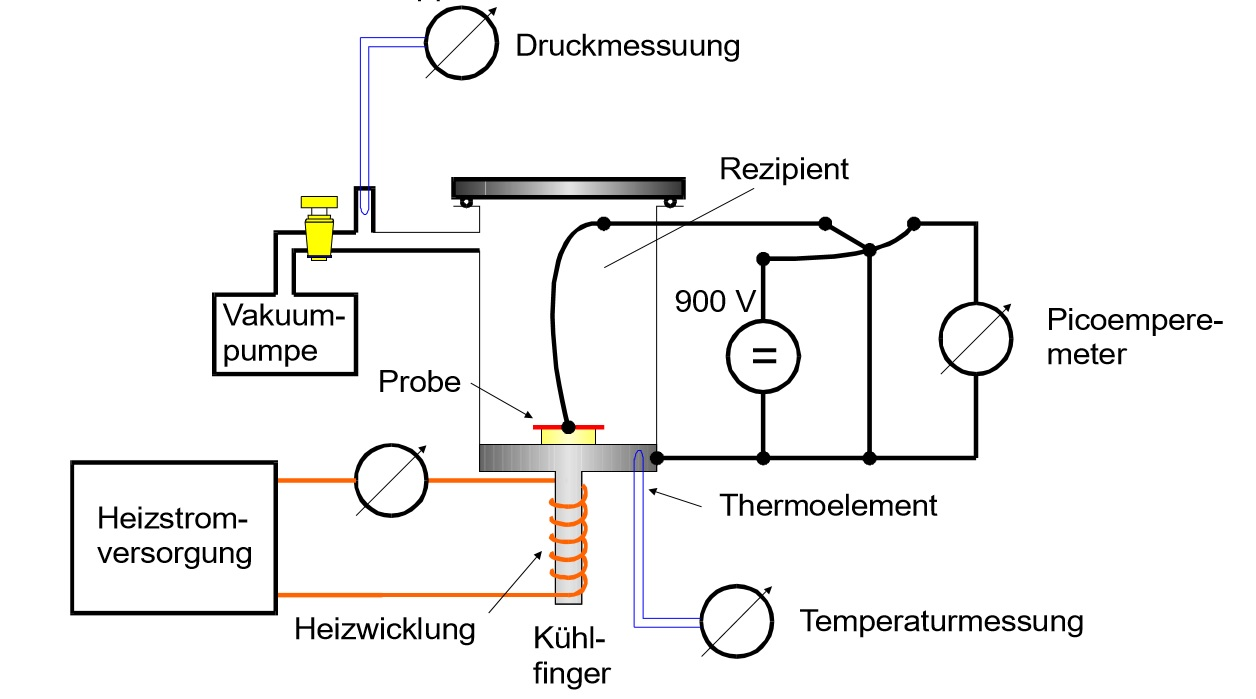
\includegraphics[scale=0.5]{content/aufbau.jpg}
\caption{Schematischer Aufbau der Versuchsapperatur \cite{Anleitung}.}
\label{fig:Aufbau}
\end{figure}